\documentclass[tikz,border=3pt]{standalone}
\usetikzlibrary{arrows.meta,calc}
\begin{document}
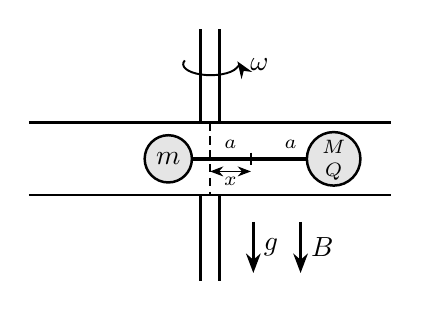
\begin{tikzpicture}[scale=1.0,>=Stealth,line width=0.9pt]
  % 回転軸（上下に分けて管の背後を通る）
  \draw (-0.12,0.46) -- (-0.12,1.65);
  \draw ( 0.12,0.46) -- ( 0.12,1.65);
  \draw (-0.12,-1.55) -- (-0.12,-0.46);
  \draw ( 0.12,-1.55) -- ( 0.12,-0.46);

  % 角周波数 omega の回転矢印（上から見て反時計回り）
  \draw[line width=0.7pt,->] (-0.32,1.25) arc[start angle=160,end angle=375,x radius=0.35,y radius=0.14];
  \node[right] at (0.38,1.20) {$\omega$};

  % 水平な管（少し上下に余裕を持たせる）
  \draw (-2.3, 0.46) -- (2.3, 0.46);
  \draw (-2.3,-0.46) -- (2.3,-0.46);

  % 質点 m, M と棒（棒の中心を x = 0.52 とする）
  \def\xc{0.52}
  \def\aa{1.05}
  \coordinate (Lm) at (\xc-\aa, 0);
  \coordinate (Cc) at (\xc, 0);
  \coordinate (RM) at (\xc+\aa, 0);

  \draw[line width=1.4pt] (Lm) -- (RM);
  \draw[fill=black!10] (Lm) circle (0.30);
  \node at (Lm) {$m$};
  \draw[fill=black!10] (RM) circle (0.34);
  \node[yshift=4.5pt] at (RM) {\scriptsize $M$};
  \node[yshift=-4.5pt] at (RM) {\scriptsize $Q$};

  % 回転軸と棒の中心の目印
  \draw[line width=0.4pt,densely dashed] (0,0.46) -- (0,-0.46);
  \draw[line width=0.4pt] (\xc,0.08) -- (\xc,-0.08);
  \draw[line width=0.4pt,<->] (0,-0.16) -- (\xc,-0.16);
  \node[below,inner sep=1.5pt] at (0.5*\xc,-0.17) {\scriptsize $x$};

  % 長さ a の表示（破線と重ならない位置に配置）
  \node[above,inner sep=1.5pt] at (0.26,0.06) {\scriptsize $a$};
  \node[above,inner sep=1.5pt] at (\xc+0.48*\aa,0.06) {\scriptsize $a$};

  % 重力と磁場（鉛直下向き）
  \draw[->] (0.55,-0.80) -- (0.55,-1.45);
  \node[right] at (0.55,-1.12) {$g$};
  \draw[->] (1.15,-0.80) -- (1.15,-1.45);
  \node[right] at (1.15,-1.12) {$B$};
\end{tikzpicture}
\end{document}
